\documentclass{standalone}
\usepackage{tikz}

\begin{document}

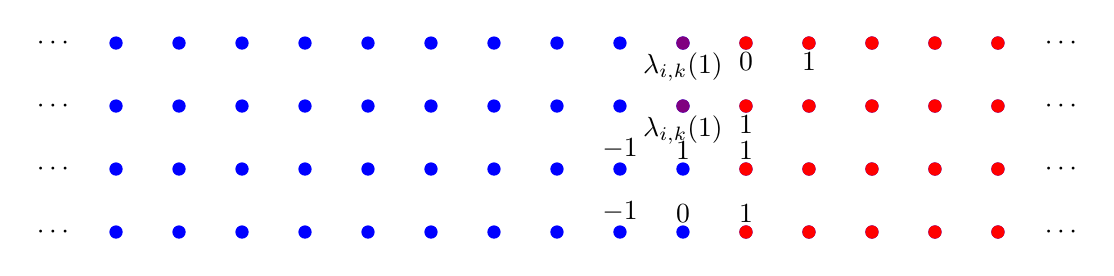
\begin{tikzpicture}[scale=0.8]

% Define colors for dots
\definecolor{blueDot}{RGB}{0, 0, 255}
\definecolor{redDot}{RGB}{255, 0, 0}
\definecolor{purpleDot}{RGB}{128, 0, 128}

% Draw the grid rows
\foreach \y in {0, 1, 2, 3} {
    \foreach \x in {-4,...,10} {
        \fill[blueDot] (\x,\y) circle (3pt);
    }
}

% Replace specific dots with red or purple
\foreach \y in {0, 1, 2, 3} {
    \fill[redDot] (6,\y) circle (3pt); % Red dot at column 6
    \fill[redDot] (7,\y) circle (3pt); % Red dot at column 7
    \fill[redDot] (8,\y) circle (3pt); % Red dot at column 8
    \fill[redDot] (9,\y) circle (3pt); % Red dot at column 9
    \fill[redDot] (10,\y) circle (3pt); % Red dot at column 10
}

% Place purple dots at specific locations
\fill[purpleDot] (5,2) circle (3pt); % Purple dot at column 5, row 2
\fill[purpleDot] (5,3) circle (3pt); % Purple dot at column 5, row 3

% Add labels
\node at (4,0) [above] {$-1$};
\node at (5,0) [above] {$0$};
\node at (6,0) [above] {$1$};

\node at (4,1) [above] {$-1$};
\node at (5,1) [above] {$1$};
\node at (6,1) [above] {$1$};

\node at (5,2) [below] {$\lambda_{i,k}(1)$};
\node at (6,2) [below] {$1$};

\node at (5,3) [below] {$\lambda_{i,k}(1)$};
\node at (6,3) [below] {$0$};
\node at (7,3) [below] {$1$};

% Add ellipses at the ends of rows
\node at (-5,0) {$\cdots$};
\node at (-5,1) {$\cdots$};
\node at (-5,2) {$\cdots$};
\node at (-5,3) {$\cdots$};
\node at (11,0) {$\cdots$};
\node at (11,1) {$\cdots$};
\node at (11,2) {$\cdots$};
\node at (11,3) {$\cdots$};

\end{tikzpicture}

\end{document}